% Options for packages loaded elsewhere
\PassOptionsToPackage{unicode}{hyperref}
\PassOptionsToPackage{hyphens}{url}
%
\documentclass[
]{article}
\usepackage{lmodern}
\usepackage{amssymb,amsmath}
\usepackage{ifxetex,ifluatex}
\ifnum 0\ifxetex 1\fi\ifluatex 1\fi=0 % if pdftex
  \usepackage[T1]{fontenc}
  \usepackage[utf8]{inputenc}
  \usepackage{textcomp} % provide euro and other symbols
\else % if luatex or xetex
  \usepackage{unicode-math}
  \defaultfontfeatures{Scale=MatchLowercase}
  \defaultfontfeatures[\rmfamily]{Ligatures=TeX,Scale=1}
\fi
% Use upquote if available, for straight quotes in verbatim environments
\IfFileExists{upquote.sty}{\usepackage{upquote}}{}
\IfFileExists{microtype.sty}{% use microtype if available
  \usepackage[]{microtype}
  \UseMicrotypeSet[protrusion]{basicmath} % disable protrusion for tt fonts
}{}
\makeatletter
\@ifundefined{KOMAClassName}{% if non-KOMA class
  \IfFileExists{parskip.sty}{%
    \usepackage{parskip}
  }{% else
    \setlength{\parindent}{0pt}
    \setlength{\parskip}{6pt plus 2pt minus 1pt}}
}{% if KOMA class
  \KOMAoptions{parskip=half}}
\makeatother
\usepackage{xcolor}
\IfFileExists{xurl.sty}{\usepackage{xurl}}{} % add URL line breaks if available
\IfFileExists{bookmark.sty}{\usepackage{bookmark}}{\usepackage{hyperref}}
\hypersetup{
  pdftitle={Ajuste de modelos preditivos com o pacote \{parsnip\}},
  pdfauthor={Edgar Cutar Junior},
  hidelinks,
  pdfcreator={LaTeX via pandoc}}
\urlstyle{same} % disable monospaced font for URLs
\usepackage[margin=1in]{geometry}
\usepackage{color}
\usepackage{fancyvrb}
\newcommand{\VerbBar}{|}
\newcommand{\VERB}{\Verb[commandchars=\\\{\}]}
\DefineVerbatimEnvironment{Highlighting}{Verbatim}{commandchars=\\\{\}}
% Add ',fontsize=\small' for more characters per line
\usepackage{framed}
\definecolor{shadecolor}{RGB}{248,248,248}
\newenvironment{Shaded}{\begin{snugshade}}{\end{snugshade}}
\newcommand{\AlertTok}[1]{\textcolor[rgb]{0.94,0.16,0.16}{#1}}
\newcommand{\AnnotationTok}[1]{\textcolor[rgb]{0.56,0.35,0.01}{\textbf{\textit{#1}}}}
\newcommand{\AttributeTok}[1]{\textcolor[rgb]{0.77,0.63,0.00}{#1}}
\newcommand{\BaseNTok}[1]{\textcolor[rgb]{0.00,0.00,0.81}{#1}}
\newcommand{\BuiltInTok}[1]{#1}
\newcommand{\CharTok}[1]{\textcolor[rgb]{0.31,0.60,0.02}{#1}}
\newcommand{\CommentTok}[1]{\textcolor[rgb]{0.56,0.35,0.01}{\textit{#1}}}
\newcommand{\CommentVarTok}[1]{\textcolor[rgb]{0.56,0.35,0.01}{\textbf{\textit{#1}}}}
\newcommand{\ConstantTok}[1]{\textcolor[rgb]{0.00,0.00,0.00}{#1}}
\newcommand{\ControlFlowTok}[1]{\textcolor[rgb]{0.13,0.29,0.53}{\textbf{#1}}}
\newcommand{\DataTypeTok}[1]{\textcolor[rgb]{0.13,0.29,0.53}{#1}}
\newcommand{\DecValTok}[1]{\textcolor[rgb]{0.00,0.00,0.81}{#1}}
\newcommand{\DocumentationTok}[1]{\textcolor[rgb]{0.56,0.35,0.01}{\textbf{\textit{#1}}}}
\newcommand{\ErrorTok}[1]{\textcolor[rgb]{0.64,0.00,0.00}{\textbf{#1}}}
\newcommand{\ExtensionTok}[1]{#1}
\newcommand{\FloatTok}[1]{\textcolor[rgb]{0.00,0.00,0.81}{#1}}
\newcommand{\FunctionTok}[1]{\textcolor[rgb]{0.00,0.00,0.00}{#1}}
\newcommand{\ImportTok}[1]{#1}
\newcommand{\InformationTok}[1]{\textcolor[rgb]{0.56,0.35,0.01}{\textbf{\textit{#1}}}}
\newcommand{\KeywordTok}[1]{\textcolor[rgb]{0.13,0.29,0.53}{\textbf{#1}}}
\newcommand{\NormalTok}[1]{#1}
\newcommand{\OperatorTok}[1]{\textcolor[rgb]{0.81,0.36,0.00}{\textbf{#1}}}
\newcommand{\OtherTok}[1]{\textcolor[rgb]{0.56,0.35,0.01}{#1}}
\newcommand{\PreprocessorTok}[1]{\textcolor[rgb]{0.56,0.35,0.01}{\textit{#1}}}
\newcommand{\RegionMarkerTok}[1]{#1}
\newcommand{\SpecialCharTok}[1]{\textcolor[rgb]{0.00,0.00,0.00}{#1}}
\newcommand{\SpecialStringTok}[1]{\textcolor[rgb]{0.31,0.60,0.02}{#1}}
\newcommand{\StringTok}[1]{\textcolor[rgb]{0.31,0.60,0.02}{#1}}
\newcommand{\VariableTok}[1]{\textcolor[rgb]{0.00,0.00,0.00}{#1}}
\newcommand{\VerbatimStringTok}[1]{\textcolor[rgb]{0.31,0.60,0.02}{#1}}
\newcommand{\WarningTok}[1]{\textcolor[rgb]{0.56,0.35,0.01}{\textbf{\textit{#1}}}}
\usepackage{longtable,booktabs}
% Correct order of tables after \paragraph or \subparagraph
\usepackage{etoolbox}
\makeatletter
\patchcmd\longtable{\par}{\if@noskipsec\mbox{}\fi\par}{}{}
\makeatother
% Allow footnotes in longtable head/foot
\IfFileExists{footnotehyper.sty}{\usepackage{footnotehyper}}{\usepackage{footnote}}
\makesavenoteenv{longtable}
\usepackage{graphicx,grffile}
\makeatletter
\def\maxwidth{\ifdim\Gin@nat@width>\linewidth\linewidth\else\Gin@nat@width\fi}
\def\maxheight{\ifdim\Gin@nat@height>\textheight\textheight\else\Gin@nat@height\fi}
\makeatother
% Scale images if necessary, so that they will not overflow the page
% margins by default, and it is still possible to overwrite the defaults
% using explicit options in \includegraphics[width, height, ...]{}
\setkeys{Gin}{width=\maxwidth,height=\maxheight,keepaspectratio}
% Set default figure placement to htbp
\makeatletter
\def\fps@figure{htbp}
\makeatother
\setlength{\emergencystretch}{3em} % prevent overfull lines
\providecommand{\tightlist}{%
  \setlength{\itemsep}{0pt}\setlength{\parskip}{0pt}}
\setcounter{secnumdepth}{-\maxdimen} % remove section numbering

\title{Ajuste de modelos preditivos com o pacote \{parsnip\}}
\author{Edgar Cutar Junior}
\date{2019-10-06}

\begin{document}
\maketitle

Neste
\href{https://www.linkedin.com/pulse/pr\%C3\%A9-processamento-de-dados-r-com-o-pacote-recipes-edgar-cutar-junior/}{segundo
post da série sobre o Tidymodels}, o conjunto de pacotes desenvolvido
por \href{twitter.com/topepos}{Max Kuhn} para ajuste de modelos
preditivos para R, iremos falar sobre o
\href{https://tidymodels.github.io/parsnip/}{\{parsnip\}}. Esse post
saiu quase todo da \href{https://tidymodels.github.io/parsnip/}{própria
página do pacote parsnip} assim como de posts do Max Kuhn no RStudio
(notadamente
\href{https://www.tidyverse.org/blog/2019/04/parsnip-internals/}{este} e
\href{https://www.tidyverse.org/blog/2018/11/parsnip-0-0-1/}{este}).
Todas as eventuais piadas ruins são minhas mesmo.

\hypertarget{cenouras-e-pastinagas}{%
\subsection{Cenouras e Pastinagas}\label{cenouras-e-pastinagas}}

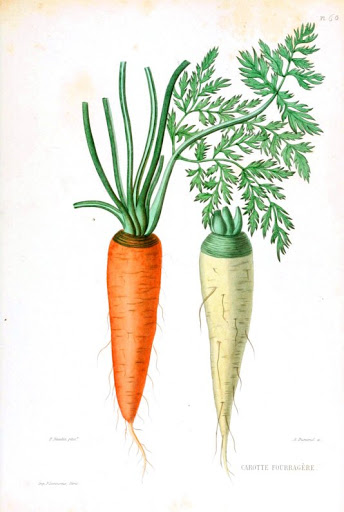
\includegraphics{Parsnip_vs_carrot.jpg}

Parsnip é o nome em inglês da pastinaga, parente esquecida da cenoura.
Originalmente parsnip era o pacote que iria substituir o
\href{http://caret.r-forge.r-project.org/}{\{caret\}} (a pronúncia de
caret é igual a ``carrot'', cenoura em inglês), que foi o primeiro
pacote integrado para modelagem preditiva para R, desenvolvido no começo
dos anos 2000 pelo mesmo Max Kuhn, na época diretor de pesquisa
não-clínica na Pfizer.

Com a evolução do pacote, a ideia originaldo Parsnip acabou se
desdobrando no conjunto de pacotes que compõem o \{tidymodels\}, cada um
deles especializado em tarefas específicas da modelagem preditiva. Com
isso
\href{https://www.tidyverse.org/blog/2018/11/parsnip-0-0-1/}{Parsnip
ficou com um problema bem específico, a interface.}

\hypertarget{uma-interface-padronizada}{%
\subsection{Uma interface padronizada}\label{uma-interface-padronizada}}

Diversas funções e pacotes oferecem diferentes interfaces e parâmetros
para objetivos parecidos, e o parsnip padroniza essa interface para o
ajuste dos modelos e também para retornar os valores preditos.

\hypertarget{o-problema}{%
\subsubsection{O Problema}\label{o-problema}}

O problema de inconsistência de interface é facilmente encontrado em
diversos modelos do R. Um exemplo simples acontece na regressão
logística. Talvez o mais consagrado modo de
\href{https://www.rdocumentation.org/packages/stats/versions/3.6.2/topics/glm}{ajustar
uma regressão logística seja através do pacote \texttt{glm}}. Esse
pacote usa a sintaxe padrão do R
(\href{https://www.amazon.com.br/dp/B07737S8XJ/ref=dp-kindle-redirect?_encoding=UTF8\&btkr=1}{que,
na verdade, precede o R}).

Para ajustar uma regressão logística no \texttt{glm} você:

\begin{itemize}
\tightlist
\item
  Usa o método da fórmula para definir as variáveis preditoras e o que
  deve ser predito.
\item
  O método da fórmula usa o formato
  \texttt{Y\ \textasciitilde{}\ X1\ +\ X2\ +\ X3}
\item
  Para especificar que é um modelo logístico usamos o argumento
  \texttt{family\ =\ binomial}
\end{itemize}

Agora vamos supor que eu queira aplicar alguma regularização nesse
modelo. Uma escolha possível seria
\href{https://cran.r-project.org/web/packages/glmnet/index.html}{usando
o pacote \texttt{glmnet}}. Nesse caso:

\begin{itemize}
\tightlist
\item
  Esse pacote não usa o método da fórmula, deve-se entregar os
  preditores em uma matriz (o que implica que variáveis ``dummy'' devem
  ser pré-computadas)
\item
  O argumento da família muda ligeiramente, e deve ser
  \texttt{family\ =\ "binomial"}
\end{itemize}

O problema seria ainda maior se eu tentasse usar a interface para o
TensorFlow no pacote \texttt{keras}. O \texttt{keras} tem uma abordagem
muito interessante para sequeciar modelos de Deep Learning mas a
formulação é completamente diferente do tradicional. Ajustar um modelo
usando \texttt{keras} exigiria estudar e entender uma outra forma de
sintaxe de modelos.

O problema se estende a como os diferentes pacotes retornam predições. A
maior parte dos pacotes em R usam a função \texttt{predict()}. Para
retornar um vetor de probabilidades na nossa regressão logística,
usaríamos \texttt{predict(obj,\ newdata,\ type\ =\ "response")}. Mas
essa convenção varia bastante entre pacotes.

\begin{longtable}[]{@{}lll@{}}
\toprule
Função & Pacote & Código\tabularnewline
\midrule
\endhead
glm & stats & predict(obj, type = ``response'')\tabularnewline
lda & MASS & predict(obj)\tabularnewline
gbm & gbm & predict(obj, type = ``response'', n.trees)\tabularnewline
mda & mda & predict(obj, type = ``posterior'')\tabularnewline
rpart & rpart & predict(obj, type = ``prob'')\tabularnewline
Weka & RWeka & predict(obj, type = ``probability'')\tabularnewline
\bottomrule
\end{longtable}

Numa instância maior, podemos ter ainda mais problemas: alguns modelos
podem criar predições em vários submodelos de uma vez. Quando usamos
Boosted Trees ajustadas com \emph{i} árvores, podemos fazer uma predição
usando menos de \emph{i} iterações (efetivamente criando um novo modelo
de predição), o que pode levar a mais inconsistências.

Esse tipo de problema, quando agregado, podia levar ao questionamento

\begin{quote}
O R está trabalhando pra mim ou eu estou trabalhando para o R?
\end{quote}

\hypertarget{a-soluuxe7uxe3o}{%
\subsubsection{A solução}\label{a-soluuxe7uxe3o}}

Para demonstrar como o \texttt{parsnip} funciona, vamos seguir com o
exemplo da regressão logística.

Para isso vamos usar uma base de dados chamada \texttt{Smarket}, do
pacote ISLR, que tem os retornos diários do índice S\&P500 entre 2001 e
2005. Vamos começar dividindo a base em treino e teste. Vamos
centralizar e escalar usando uma receita simples do pacote
\texttt{recipes}\href{(https://www.linkedin.com/pulse/pr\%C3\%A9-processamento-de-dados-r-com-o-pacote-recipes-edgar-cutar-junior/)}{(falamos
sobre esse pacote no último post)}{]}.

\begin{Shaded}
\begin{Highlighting}[]
\ControlFlowTok{if}\NormalTok{ (}\OperatorTok{!}\KeywordTok{require}\NormalTok{(}\StringTok{"pacman"}\NormalTok{)) }\KeywordTok{install.packages}\NormalTok{(}\StringTok{"pacman"}\NormalTok{)}
\end{Highlighting}
\end{Shaded}

\begin{verbatim}
## Loading required package: pacman
\end{verbatim}

\begin{Shaded}
\begin{Highlighting}[]
\NormalTok{pacman}\OperatorTok{::}\KeywordTok{p_load}\NormalTok{(tidymodels, ISLR) }

\NormalTok{split <-}\StringTok{ }\KeywordTok{initial_split}\NormalTok{(Smarket }\OperatorTok\StringTok{ }\KeywordTok{select}\NormalTok{(}\OperatorTok{-}\NormalTok{Year, }\OperatorTok{-}\NormalTok{Today), }\DataTypeTok{props =} \DecValTok{9}\OperatorTok{/}\DecValTok{10}\NormalTok{)}
\NormalTok{smarket_train <-}\StringTok{ }\KeywordTok{training}\NormalTok{(split)}
\NormalTok{smarket_test  <-}\StringTok{ }\KeywordTok{testing}\NormalTok{(split)}

\NormalTok{smarket_rec <-}\StringTok{ }\KeywordTok{recipe}\NormalTok{(Direction }\OperatorTok{~}\StringTok{ }\NormalTok{., }\DataTypeTok{data =}\NormalTok{ smarket_train) }\OperatorTok
\StringTok{  }\KeywordTok{step_center}\NormalTok{(}\KeywordTok{all_predictors}\NormalTok{()) }\OperatorTok
\StringTok{  }\KeywordTok{step_scale}\NormalTok{(}\KeywordTok{all_predictors}\NormalTok{()) }\OperatorTok
\StringTok{  }\KeywordTok{prep}\NormalTok{(}\DataTypeTok{training =}\NormalTok{ smarket_train, }\DataTypeTok{retain =} \OtherTok{TRUE}\NormalTok{)}

\NormalTok{train_data <-}\StringTok{ }\KeywordTok{juice}\NormalTok{(smarket_rec)}
\NormalTok{test_data  <-}\StringTok{ }\KeywordTok{bake}\NormalTok{(smarket_rec, smarket_test)}
\end{Highlighting}
\end{Shaded}

Para usar o \texttt{parsnip}, você começa com a especificação de um
modelo. É um objeto simples que define a intenção daquele modelo. Já que
vamos seguir com nossa saga de regressão logística, nosso primeiro passo
é uma função simples.

\begin{Shaded}
\begin{Highlighting}[]
\NormalTok{market_model <-}\StringTok{ }\KeywordTok{logistic_reg}\NormalTok{()}
\NormalTok{market_model}
\end{Highlighting}
\end{Shaded}

\begin{verbatim}
## Logistic Regression Model Specification (classification)
\end{verbatim}

Pode parecer estranho porque não entramos com absolutamente nenhum
detalhe sobre o que vamos fazer, mas é isso aí mesmo! O \texttt{parsnip}
oferece uma variedade de formas para ajustar esse modelo. Nós vamos usar
o tradicional Método dos Mínimos Quadrados, mas poderia ser com
penalização (via lasso, ridge, Bayes etc)\ldots{} Diferenciamos um caso
do outro através da \emph{\emph{Engine} computacional}, que é uma
combinação de tipo de estimação com implementação. Pode ser através de
um pacote ou uma plataforma como Spark ou TensorFlow. Para começar
simples, vamos usar o glm.

\begin{Shaded}
\begin{Highlighting}[]
\NormalTok{glm_market_model <-}\StringTok{ }\NormalTok{market_model }\OperatorTok\StringTok{ }\KeywordTok{set_engine}\NormalTok{(}\StringTok{"glm"}\NormalTok{)}
\NormalTok{glm_market_model}
\end{Highlighting}
\end{Shaded}

\begin{verbatim}
## Logistic Regression Model Specification (classification)
## 
## Computational engine: glm
\end{verbatim}

Não existem mais muitos argumentos por aqui, então vamos pular direto
pro ajuste do modelo. Nossas duas escolhas nesse ponto são entre usar
\texttt{fit()} ou \texttt{fit\_xy()}. O primeiro usa o método da
fórmula, enquanto o segundo usa objetos separados para os preditores e
para o resultado.

\begin{Shaded}
\begin{Highlighting}[]
\NormalTok{glm_fit <-}\StringTok{ }\NormalTok{glm_market_model }\OperatorTok
\StringTok{  }\KeywordTok{fit}\NormalTok{(Direction }\OperatorTok{~}\StringTok{ }\NormalTok{., }\DataTypeTok{data =}\NormalTok{ train_data)}

\CommentTok{#ou}

\NormalTok{glm_market_model }\OperatorTok
\StringTok{  }\KeywordTok{fit_xy}\NormalTok{(}\DataTypeTok{x =} \KeywordTok{select}\NormalTok{(train_data, }\OperatorTok{-}\NormalTok{Direction), }\DataTypeTok{y =} \KeywordTok{select}\NormalTok{(train_data, Direction))}
\end{Highlighting}
\end{Shaded}

\begin{verbatim}
## parsnip model object
## 
## Fit time:  0ms 
## 
## Call:  stats::glm(formula = formula, family = stats::binomial, data = data)
## 
## Coefficients:
## (Intercept)         Lag1         Lag2         Lag3         Lag4         Lag5  
##     0.01712     -0.05378     -0.02495      0.04106      0.08615      0.04467  
##      Volume  
##     0.06600  
## 
## Degrees of Freedom: 937 Total (i.e. Null);  931 Residual
## Null Deviance:       1300 
## Residual Deviance: 1296  AIC: 1310
\end{verbatim}

Claro que não é necessário fazer todos esses passos individualmente, e
poderíamos simplesmente condensar tudo em um só objeto.

\begin{Shaded}
\begin{Highlighting}[]
\NormalTok{glm_fit <-}\StringTok{ }\KeywordTok{logistic_reg}\NormalTok{() }\OperatorTok\StringTok{ }
\StringTok{  }\KeywordTok{set_engine}\NormalTok{(}\StringTok{"glm"}\NormalTok{) }\OperatorTok\StringTok{ }
\StringTok{  }\KeywordTok{fit}\NormalTok{(Direction }\OperatorTok{~}\StringTok{ }\NormalTok{., }\DataTypeTok{data =}\NormalTok{ train_data)}
\end{Highlighting}
\end{Shaded}

\hypertarget{mais-engines}{%
\subsubsection{Mais engines!}\label{mais-engines}}

O valor do \texttt{parsnip} começa quando queremos testar diferentes
\emph{engines}. Vamos usar o mesmo modelo e estimar os coeficientes
através de estimativa Bayesiana usando \texttt{stan}. Para isso só
precisamos:

\begin{Shaded}
\begin{Highlighting}[]
\NormalTok{stan_model <-}\StringTok{ }\KeywordTok{logistic_reg}\NormalTok{() }\OperatorTok\StringTok{ }
\StringTok{  }\KeywordTok{set_engine}\NormalTok{(}\StringTok{"stan"}\NormalTok{)}

\NormalTok{stan_model}
\end{Highlighting}
\end{Shaded}

\begin{verbatim}
## Logistic Regression Model Specification (classification)
## 
## Computational engine: stan
\end{verbatim}

Para ajustar esse modelo, o \texttt{parsnip} chamou a função
\texttt{stan\_glm()} do pacote \texttt{rstanarm}. Se você quiser passar
argumentos para essa função, simplesmente adicione eles na função
\texttt{set\_engine()}:

\begin{Shaded}
\begin{Highlighting}[]
\NormalTok{stan_model <-}\StringTok{ }\KeywordTok{logistic_reg}\NormalTok{() }\OperatorTok\StringTok{ }
\StringTok{  }\KeywordTok{set_engine}\NormalTok{(}\StringTok{"stan"}\NormalTok{, }\DataTypeTok{iter =} \DecValTok{5000}\NormalTok{) }

\NormalTok{stan_model}
\end{Highlighting}
\end{Shaded}

\begin{verbatim}
## Logistic Regression Model Specification (classification)
## 
## Engine-Specific Arguments:
##   iter = 5000
## 
## Computational engine: stan
\end{verbatim}

O modelo pode ser ajustado da mesma forma. \texttt{rstanarm} printa
\emph{MUITAS} informações ao ajustar um modelo. Isso pode ser útil para
diagnóstico mas vamos excluir usando uma função de controle.

\begin{Shaded}
\begin{Highlighting}[]
\NormalTok{ctrl <-}\StringTok{ }\KeywordTok{fit_control}\NormalTok{(}\DataTypeTok{verbosity =} \DecValTok{0}\NormalTok{)}

\NormalTok{stan_fit <-}\StringTok{ }\NormalTok{stan_model }\OperatorTok
\StringTok{    }\KeywordTok{fit}\NormalTok{(Direction }\OperatorTok{~}\StringTok{ }\NormalTok{., }\DataTypeTok{data =}\NormalTok{ train_data, }\DataTypeTok{control =}\NormalTok{ ctrl)}

\NormalTok{stan_fit}
\end{Highlighting}
\end{Shaded}

\begin{verbatim}
## parsnip model object
## 
## Fit time:  7.1s 
## stan_glm
##  family:       binomial [logit]
##  formula:      Direction ~ .
##  observations: 938
##  predictors:   7
## ------
##             Median MAD_SD
## (Intercept)  0.0    0.1  
## Lag1        -0.1    0.1  
## Lag2         0.0    0.1  
## Lag3         0.0    0.1  
## Lag4         0.1    0.1  
## Lag5         0.0    0.1  
## Volume       0.1    0.1  
## 
## ------
## * For help interpreting the printed output see ?print.stanreg
## * For info on the priors used see ?prior_summary.stanreg
\end{verbatim}

\hypertarget{prediuxe7uxf5es}{%
\subsubsection{Predições}\label{prediuxe7uxf5es}}

Além das óbvias funcionalidades para ajustar diferentes modelos, ainda
temos muitas vantagens na hora de prever resultados. Isso resolve uma
série de frustrações como ter um arquivo predito que PULA algum
resultado quando tem valores faltando, por exemplo, além de padronizar a
função.

Para regressões logísticas, por exemplo, o output é sempre um
\texttt{tibble} com uma coluna \texttt{.pred\_class} contendo a classe
predita.

\begin{Shaded}
\begin{Highlighting}[]
\KeywordTok{predict}\NormalTok{(glm_fit, test_data)}
\end{Highlighting}
\end{Shaded}

\begin{verbatim}
## # A tibble: 312 x 1
##    .pred_class
##    <fct>      
##  1 Down       
##  2 Down       
##  3 Up         
##  4 Up         
##  5 Down       
##  6 Down       
##  7 Down       
##  8 Down       
##  9 Up         
## 10 Up         
## # ... with 302 more rows
\end{verbatim}

\begin{Shaded}
\begin{Highlighting}[]
\KeywordTok{predict}\NormalTok{(stan_fit, test_data)}
\end{Highlighting}
\end{Shaded}

\begin{verbatim}
## # A tibble: 312 x 1
##    .pred_class
##    <fct>      
##  1 Down       
##  2 Down       
##  3 Up         
##  4 Up         
##  5 Down       
##  6 Down       
##  7 Down       
##  8 Down       
##  9 Up         
## 10 Up         
## # ... with 302 more rows
\end{verbatim}

Isso facilita a união com os valores originais e o \texttt{.} no nome é
para evitar nomes duplicados.

\texttt{parsnip} também trás diferentes tipos de previsão com uma
interface padrão. Por exemplo, para estimativa de intervalos.

\begin{Shaded}
\begin{Highlighting}[]
\KeywordTok{predict}\NormalTok{(glm_fit, test_data, }\DataTypeTok{type =} \StringTok{"conf_int"}\NormalTok{)}
\end{Highlighting}
\end{Shaded}

\begin{verbatim}
## # A tibble: 312 x 4
##    .pred_lower_Down .pred_upper_Down .pred_lower_Up .pred_upper_Up
##               <dbl>            <dbl>          <dbl>          <dbl>
##  1            0.348            0.665          0.335          0.652
##  2            0.448            0.574          0.426          0.552
##  3            0.426            0.546          0.454          0.574
##  4            0.431            0.565          0.435          0.569
##  5            0.476            0.585          0.415          0.524
##  6            0.433            0.628          0.372          0.567
##  7            0.432            0.584          0.416          0.568
##  8            0.472            0.617          0.383          0.528
##  9            0.368            0.546          0.454          0.632
## 10            0.362            0.595          0.405          0.638
## # ... with 302 more rows
\end{verbatim}

Ou para as probabilidades de cada previsão:

\begin{Shaded}
\begin{Highlighting}[]
\KeywordTok{predict}\NormalTok{(glm_fit, test_data, }\DataTypeTok{type =} \StringTok{"prob"}\NormalTok{)}
\end{Highlighting}
\end{Shaded}

\begin{verbatim}
## # A tibble: 312 x 2
##    .pred_Down .pred_Up
##         <dbl>    <dbl>
##  1      0.507    0.493
##  2      0.511    0.489
##  3      0.486    0.514
##  4      0.498    0.502
##  5      0.531    0.469
##  6      0.532    0.468
##  7      0.508    0.492
##  8      0.545    0.455
##  9      0.456    0.544
## 10      0.478    0.522
## # ... with 302 more rows
\end{verbatim}

\hypertarget{pruxf3ximos-passos}{%
\subsection{Próximos passos}\label{pruxf3ximos-passos}}

Esse artigo apenas toca a superfície das possibilidades de uso do pacote
\texttt{parsnip}. Nos próximos artigos vamos explorar como fazer uma
\emph{grid search} pelos melhores parâmetros, como fazer uma
\emph{k-fold Cross Validation} usando esta interface e como avaliar a
performance de modelos, tudo isso usando os tidymodels.

\end{document}
